\section{Humanoid Robot NAO}

We chose the torso and arms only version (T14) of the commercially available humanoid robot NAO from Aldebaran Robotics as our robotic prompting agent.  NAO is a humanoid robot about half a meter high in torso (see Figure \ref{fig:NAOColor}).  It is designed by Aldebaran Robotics to primarily serve academic researches in robotics.  NAO is equipped with the state of the art mechanical, electrical, embedded, control, and local network communication systems.  It also has cameras and sonar sensors for computer vision algorithms for scene understanding, path planning, and obstacle avoidance.  The software development kit (SDK) provided is very easy and powerful to program with.  Also, an even easier graphic user interface (GUI) for robot behavior programming, the Choreographe software, is also available.  One caveat of using NAO for SAR HRI researches is that it is only equipped with a single degree of freedom finger dexterity, though other joints in its body are much more mobile.  It is more than enough for doing simple pointing and other non-contact gestural prompts in sync with verbal interactions.  It just cannot perform detailed hand gesturing.  This makes NAO less capable in demonstrating a hand-washing step in high detail.
\begin{figure} [h]
	\centering
	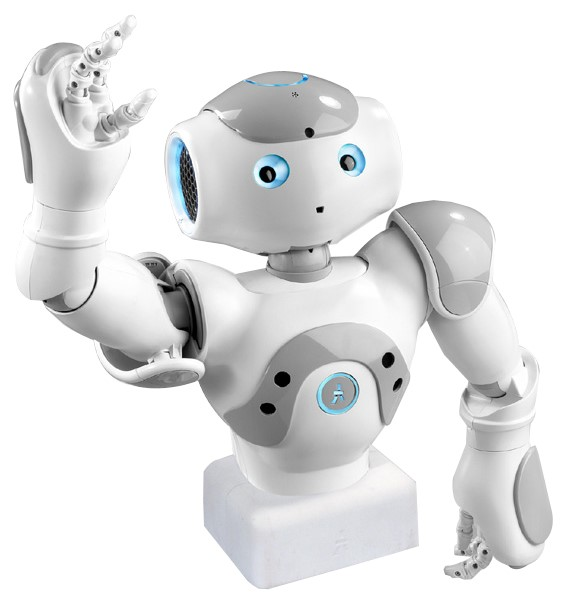
\includegraphics[width=0.6\textwidth]{./img/nao-torso.jpg}
	\caption{NAO T14 Humanoid Torso}
	\label{fig:NAOColor}
\end{figure}


From a HRI research perspective, Aldebaran Robotics took care of designing the intrinsics level of HRI, where NAO has a likable appearance and child like neutral gender voice, although it's incapable of facial expressions.  The design decisions we face when using NAO for this thesis is on the behavior level of HRI.  Design decisions such as voice intonation choice, verbal prompts, motion gestures and gaze, and eye blinks using LEDs in eye regions are made in this thesis.  The objective of this thesis is then to ultimately find out if the lower two levels of design decisions made are able to cumulate to the child with ASD perceiving NAO as a role model / supervisor / assistant during hand-washing.

For our pilot study, we use the half-torso version of NAO because we do not require any mobility from NAO -- it is fixed on the sink table top (see Figure \ref{fig:ExpSetup}).  The relevant functionalities of NAO we utilized for delivering prompts include:
\begin{itemize}
	\item Verbal prompting through its bilateral loud speakers on the head and speech synthesis functionality
	\item Body gesturing through its moving head and arms (although its fingers are not capable of hand gesturing)
	\item Flashing LEDs on the eyes and ears
\end{itemize}
\begin{figure} [h]
	\centering
	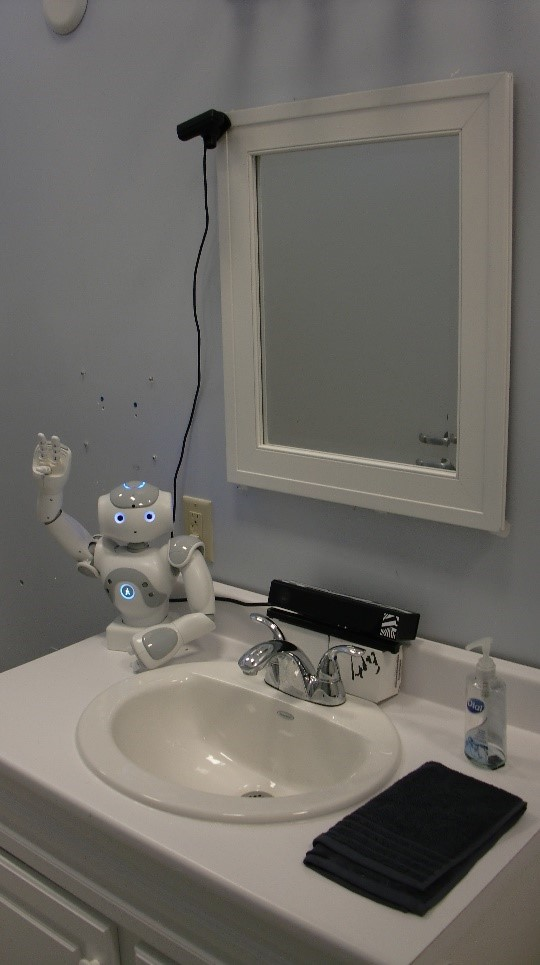
\includegraphics[height=15cm, keepaspectratio]{./img/exp_setup.jpg}
	\caption{Experiment Setup}
	\label{fig:ExpSetup}
\end{figure}


\subsection{Verbal Prompts}
We used the text-to-speech engine from NAO to synthesize the verbal prompts.  The pitch of NAO's voice was changed to a lower one than default for the verbal prompts to give a more authoritative feeling.  The reward verbal prompt remained the default pitch, though, to give an exciting praise.  The verbal prompts were worded as short, three or four words phrases, such as "turn on the water" or "rinse your hand", and a pause is put between the action and the subject so that the prompts sounded clearer and was easier to understand to children with ASD.  The specific choices of verbal and gesture prompts are discussed in Section \ref{sec:SpecificProtocol}.

\subsection{Gesture Prompts}
There are several kinds of gesture prompts NAO needs to perform:

\begin{itemize}
	\item \textbf{Attention grabber (AG)}:  When prompting is needed but the child is not looking at NAO, NAO waves to grab the child’s attention.
	\item \textbf{Motion demonstrating prompt (MoDemo)}:  NAO demonstrates to child the motion of interaction (e.g. turning tap, scrubbing, rinsing, etc.).
	\item \textbf{Object pointing prompt (ObjPt)}:  NAO points to the physical object of interaction.
	\item \textbf{Reward (REW)}:  After a task is successfully completed, NAO flashes LEDs as a positive reinforcement.
\end{itemize}

The gaze behaviour of NAO during gesture prompts is also important and is grouped as: looking at child (when delivering AG, MoDemo, REW), and looking at object (AR, ObjPt).  The gesture and gaze motions can be programmed using NAO's software, Choregraphe.

\subsection{Wizard of Oz Remote Control}
The WoZ experiment setup involves controlling the robot remotely behind the scene by a human operator, the wizard.  A touch screen laptop was used as the user interface for the operator, and the behaviors of the robot were presented as buttons on the screen, with the camera views displayed along side.  Keyboard shortcuts were also implemented for faster access to robot actions.
